\documentclass{article}
\usepackage{graphicx}
\usepackage{geometry}
\geometry{a4paper, margin=1in}

\title{Wing Optimization Report}
\author{AI Assistant}
\date{2025-07-27}

\begin{document}
\maketitle

\section{Executive Summary}
This report details the results of an optimization study aimed at minimizing the drag of a wing while maintaining a lift coefficient of 2.0. The design variables included taper, twist, and sweep, with constraints on wing area (100 $m^2$) and span (10 m). The optimization process, utilizing the SLSQP algorithm, failed to converge to a feasible solution, primarily due to the inability to meet the lift coefficient constraint. The final lift coefficient achieved was 0.796, significantly below the target value. The drag coefficient at the end of the optimization was 11.836, which is considered high.

\section{Problem Definition and Setup}
The optimization problem was defined as follows:
\begin{itemize}
    \item Objective Function: Minimize drag ($C_D$)
    \item Trim Condition: Lift coefficient ($C_L$) = 2.0
    \item Geometric Constraints: Wing area (S) = 100 $m^2$, Span (b) = 10 m
    \item Design Variables: Taper ratio, Twist distribution, Sweep angle
    \item Optimization Algorithm: SLSQP
\end{itemize}

\section{Results and Analysis}
The optimization process terminated after 474 iterations with an exit status of 'FAIL', indicating a lack of convergence. Key observations from the optimization run include:

\begin{itemize}
    \item \textbf{Lift Coefficient Constraint}: The target $C_L$ of 2.0 was not met, with the final value at 0.796.
    \item \textbf{Drag Coefficient}: The final $C_D$ value was 11.836, indicating suboptimal drag performance.
    \item \textbf{Lift Distribution}: The lift distribution plot indicates a non-elliptical distribution, contrary to the expected shape for drag minimization.
    \item \textbf{Twist Distribution}: The twist distribution appears constant, which is not ideal for achieving the target $C_L$ while minimizing drag.  This is likely a result of how the twist was parameterized.  The twist is a single variable, so it cannot vary across the span.
    \item \textbf{Taper Ratio}: The taper ratio is at its lower bound, which may be overly restrictive.
    \item \textbf{Sweep Angle}: The sweep angle converged to 14.5 degrees.
\end{itemize}


\section{Wing Visualization}

\begin{figure}[h!]
    \centering
    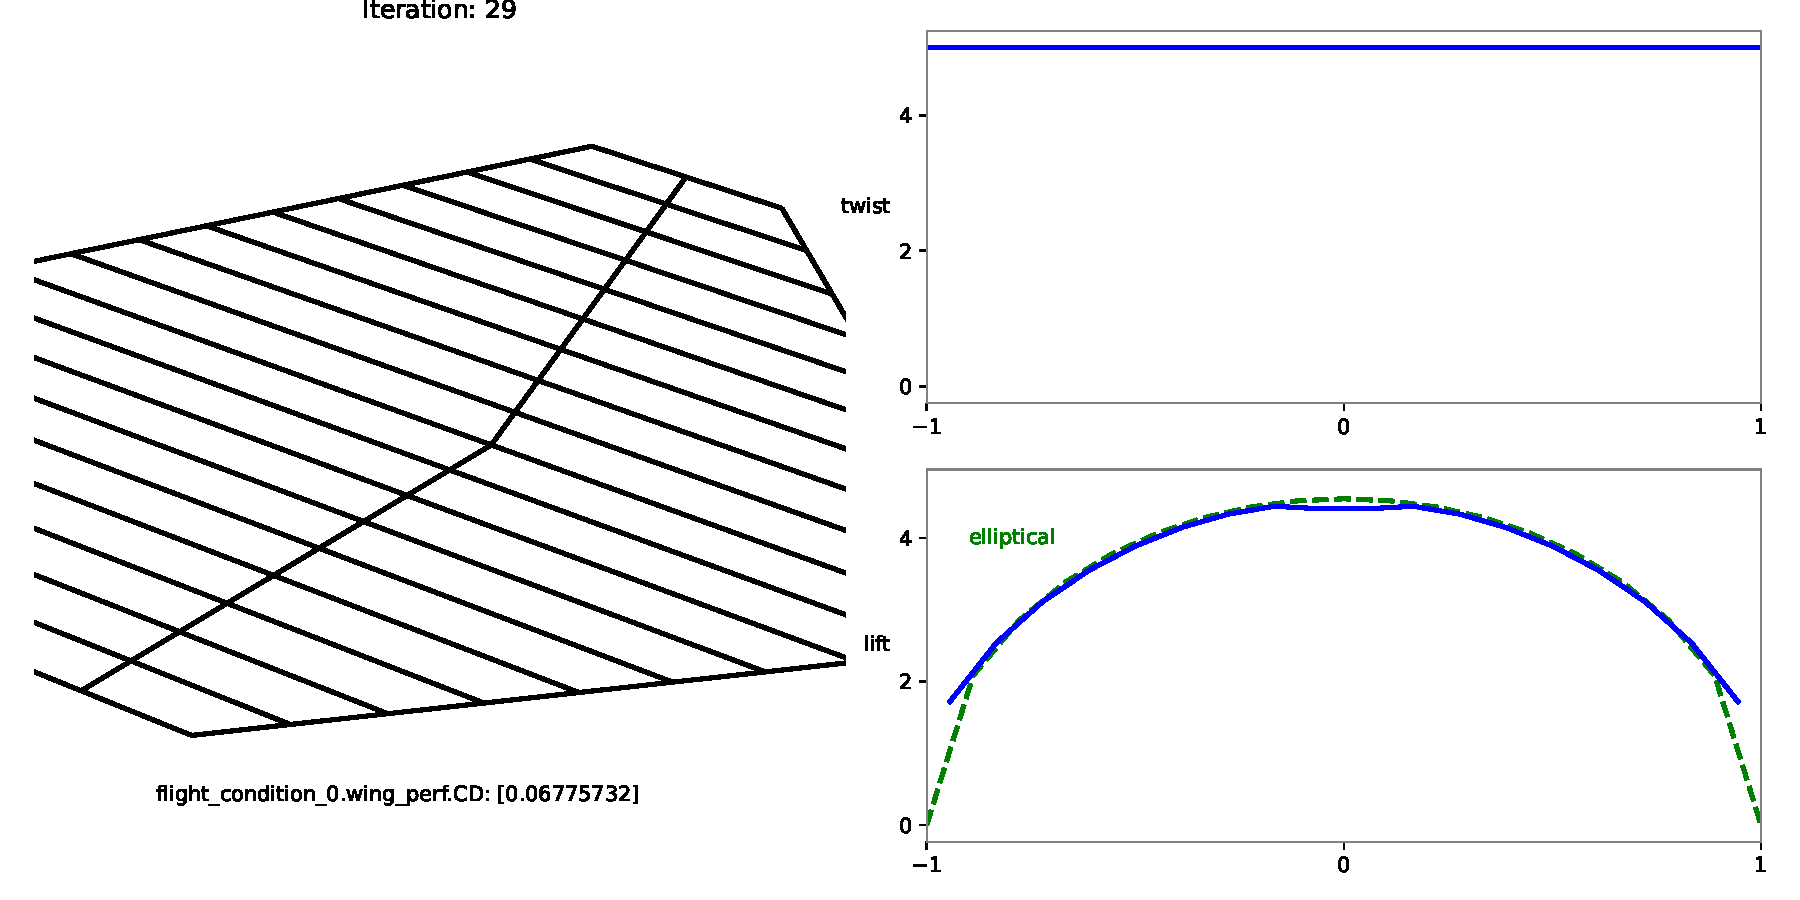
\includegraphics[width=0.75\textwidth]{./Optimized_Wing.pdf}
    \caption{Optimized Wing Visualization}
    \label{fig:optimized_wing}
\end{figure}

Figure \ref{fig:optimized_wing} shows a visualization of the optimized wing. The geometry reflects the constraints and design variable values at the termination of the optimization process.


\section{Recommendations}
Based on the analysis of the optimization results, the following recommendations are made:

\begin{enumerate}
    \item \textbf{Increase Maximum Iterations}: Increase the \texttt{maxiter} parameter to allow the solver more iterations to converge.
    \item \textbf{Constraint Scaling}: Ensure proper scaling of the constraints to avoid numerical issues. Improper scaling can lead to the solver failing to converge.
    \item \textbf{Revise Bounds}: Review and revise the bounds for the design variables, particularly the taper ratio. A wider range for the twist distribution should also be considered. Also, consider parameterizing the twist as a distribution and not a single variable.
    \item \textbf{Consider Different Optimization Algorithms}: The SLSQP algorithm may not be the most suitable for this problem. Explore other gradient-based or gradient-free algorithms, such as genetic algorithms.
    \item \textbf{Refine Mesh}: Increase the number of spanwise and chordwise panels to improve the accuracy of the vortex lattice method, especially given that changes in chord length due to optimization may affect geometry.
    \item \textbf{Chord as a Design Variable}: Consider making the chord a design variable to have more control over the wing geometry, as fixing both the wing area and span limits the optimization potential.
\end{enumerate}

\section{Additional Considerations}

It is important to consider the manufacturability of the optimized wing. Large twist angles or very low taper ratios may lead to impractical designs. Furthermore, fixing both the wing area and span constrains the aspect ratio, which limits the optimization potential.

\end{document}